\section{向量的内积与向量空间}

\subsection{向量的内积}

\begin{definition}[向量的内积]
    给定 $ \mathbb{R}^{n} $ 中的向量
    $$\vb*{\alpha}=\left(a_{1}, a_{2}, \cdots, a_{n}\right)^{\top}, \quad \vb*{\beta}=\left(b_{1}, b_{2}, \cdots, b_{n}\right)^{\top}$$
    则称 $\displaystyle \sum_{i=1}^{n} a_{i} b_{i} $ 为向量 $ \vb*{\alpha} $ 与 $ \vb*{\beta} $ 的\textit{内积}, 记为 $ (\vb*{\alpha}, \vb*{\beta}) $, 即 $ \displaystyle(\vb*{\alpha}, \vb*{\beta})=\vb*{\alpha}^{\top} \vb*{\beta}=\sum_{i=1}^{n} a_{i} b_{i} $.
\end{definition}

内积具有下列性质:
\begin{enumerate}[label=(\arabic{*})]
    \item $(\vb*{\alpha}, \vb*{\beta})=(\vb*{\beta}, \vb*{\alpha}) $;
    \item $(k \vb*{\alpha}, \vb*{\beta})=k(\vb*{\alpha}, \vb*{\beta}) $;
    \item $(\vb*{\alpha}+\vb*{\beta}, \vb*{\gamma})=(\vb*{\alpha}, \vb*{\gamma})+(\vb*{\beta}, \vb*{\gamma}) $;
    \item $(\vb*{\alpha}, \vb*{\alpha}) \geqslant 0 $, 当且仅当 $ \vb*{\alpha}=\vb*{0} $ 时, 等号成立.
\end{enumerate}

\begin{definition}[向量的范数]
    如果向量 $\vb*{x}\in \mathbb{R}^{n}$ 的某个实值函数 $N(\vb*{x})=\norm{x}$, 满足以下条件:
    \begin{enumerate}[label=(\arabic{*})]
        \item $\norm{\vb*{x}}\geqslant 0$, iff $\vb*{x}=\vb*{0}$ 取等 (正定条件);
        \item $\norm{\alpha\vb*{x}}=|\alpha|\norm{\vb*{x}},~\forall a\in \mathbb{R}$ (齐次性);
        \item $\norm{\vb*{x}+\vb*{y}}\leqslant \norm{\vb*{x}}+\norm{\vb*{y}}$ (三角不等式).
    \end{enumerate}
    则称 $N(\vb*{x})$ 是 $\mathbb{R}^{n}$ 上的一个\textit{向量范数} (或\textit{模}). 由 (3) 可推出不等式: $|~\norm{\vb*{x}}-\norm{\vb*{y}}~|\leqslant \norm{\vb*{x}-\vb*{y}}$.
\end{definition}

\begin{definition}[最大范数]
    向量的 $\infty$-范数 (最大范数):
    $\displaystyle 
    \norm{\vb*{x}}_{\infty}=\max\limits_{1\leqslant i\leqslant n}|x_i|.
    $
\end{definition}

\begin{definition}[1-范数]
    向量的 1-范数: $ \displaystyle \norm{\vb*{x}}_1=\sum_{i=1}^{n} |x_i| $.
\end{definition}

\begin{definition}[2-范数]
    向量的 2-范数: $ \displaystyle \norm{\vb*{x}}_2=(\vb*{x},\vb*{x})^{\frac{1}{2}} =\qty(\sum_{i=1}^{n} x_i^2)^{\frac{1}{2}}$.
\end{definition}

\begin{definition}[$p$-范数]
    向量的 $p$-范数: $ \displaystyle \norm{\vb*{x}}_{p}=\qty(\sum_{i=1}^{n} |x_i|^p)^{\frac{1}{p}} $.
\end{definition}

\begin{theorem}[向量范数的等价性]
    设 $\norm{\vb*{x}}_s,~\norm{\vb*{x}}_t$ 为 $\mathbb{R}^{n}$ 上向量的任意两种范数, 则存在常数 $c_1,~c_2>0$, 使得 $\forall \vb*{x}\in \mathbb{R}^{n}$ 有 $$
    c_1\norm{\vb*{x}}_s\leqslant \norm{\vb*{x}}_t\leqslant c_2\norm{\vb*{x}}_s.
    $$
\end{theorem}

% 向量范数具有下列性质:
% \begin{enumerate}[label=(\arabic{*})]
%     \item $\|\vb*{\alpha}\| \geqslant 0  $, 当且仅当 $ \vb*{\alpha}=\vb*{0} $ 时, 等号成立;
%     \item 对于任意向量 $ \vb*{\alpha} $ 和任意实数 $ k $, 都有 $ \|k \vb*{\alpha}\|=|k|\|\vb*{\alpha}\| $;
%     \item 对于任意 $ n $ 维向量 $ \vb*{\alpha} $ 和 $ \vb*{\beta} $, 有 $ |(\vb*{\alpha}, \vb*{\beta})|=\left|\vb*{\alpha}^{\top} \vb*{\beta}\right| \leqslant\|\vb*{\alpha}\| \cdot\|\vb*{\beta}\|$.
% \end{enumerate}

\begin{definition}[向量的正交]
    如果向量 $ \vb*{\alpha} $ 和 $ \vb*{\beta} $ 的内积等于零, 即 $ (\vb*{\alpha}, \vb*{\beta})=0 $, 则称  $\vb*{\alpha} $ 和 $ \vb*{\beta} $ \textit{相互正交}. 如果非零向量组 $ \vb*{\alpha}_{1}, \vb*{\alpha}_{2}, \cdots, \vb*{\alpha}_{s} $ 中的向量两两正交, 即 $ \left(\vb*{\alpha}_{i}, \vb*{\alpha}_{j}\right)=0(i \neq j, i, j=1 ,  2, \cdots, s) $, 则称该向量组为\textit{正交向量组}.
\end{definition}

正交向量具有下列性质:
\begin{enumerate}[label=(\arabic{*})]
    \item 零向量与任何向量正交;
    \item 与自己正交的向量只有零向量;
    \item 正交向量组是线性无关的;
    \item 对任意向量 $ \vb*{\alpha} $ 和 $ \vb*{\beta} $, 有三角不等式
          $$\|\vb*{\alpha}+\vb*{\beta}\| \leqslant\|\vb*{\alpha}\|+\|\vb*{\beta}\|$$
          当且仅当 $ \vb*{\alpha} $ 与 $ \vb*{\beta} $ 相互正交时, 有 $ \|\vb*{\alpha}+\vb*{\beta}\|^{2}=\|\vb*{\alpha}\|^{2}+\|\vb*{\beta}\|^{2} $.
\end{enumerate}

\begin{definition}[初等反射矩阵]
    设向量 $\vb*{w}\in \mathbb{R}^{n}$, 且 $\vb*{w}^\top\vb*{w}=1$, 称矩阵 $\vb*{H}=\vb*{E}-2\vb*{ww}^\top$ 为\textit{初等反射矩阵}, 也称为 \textit{Householder 变换}.
\end{definition}

设有初等反射矩阵 $\vb*{H}=\vb*{E}-2\vb*{ww}^\top$, 其中 $\vb*{w}^\top\vb*{w}=1$, 则 
\begin{multicols}{2}
    \begin{enumerate}[label=(\arabic{*})]
        \item $|\vb*{H}|=-1$;
        \item $\vb*{H}$ 是对称矩阵, 即 $\vb*{H}^\top=\vb*{H}$;
        \item $\vb*{H}$ 是正交矩阵, 即 $\vb*{H}^{-1}=\vb*{H}$;
        \item $\vb*{H}$ 是对合矩阵, 即 $\vb*{H}^2=\vb*{E}$;
        \item 设 $\vb*{A}$ 是对称矩阵, 则 $\vb*{A}_1=\vb*{H}^{-1}\vb*{AH}=\vb*{H}^\top\vb*{AH}$ 亦是对称矩阵.
    \end{enumerate}
    \tikzset{every picture/.style={line width=0.75pt}} %set default line width to 0.75pt        
\begin{figure}[H]
    \centering
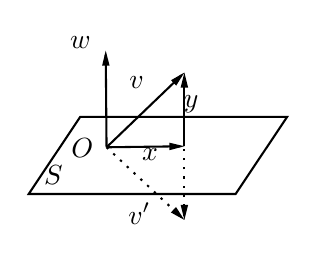
\begin{tikzpicture}[x=0.75pt,y=0.75pt,yscale=-1,xscale=1]
%uncomment if require: \path (0,310); %set diagram left start at 0, and has height of 310

%Shape: Parallelogram [id:dp04316432985707386] 
\draw   (96.11,115) -- (195.8,115) -- (170.99,152.15) -- (71.3,152.15) -- cycle ;
%Straight Lines [id:da2353302515023421] 
\draw    (108.8,129.65) -- (108.42,85.1) ;
\draw [shift={(108.4,83.1)}, rotate = 89.51] [fill={rgb, 255:red, 0; green, 0; blue, 0 }  ][line width=0.08]  [draw opacity=0] (7.2,-1.8) -- (0,0) -- (7.2,1.8) -- cycle    ;
%Straight Lines [id:da14913951087141797] 
\draw    (108.8,129.65) -- (144.3,129.18) ;
\draw [shift={(146.3,129.15)}, rotate = 179.24] [fill={rgb, 255:red, 0; green, 0; blue, 0 }  ][line width=0.08]  [draw opacity=0] (7.2,-1.8) -- (0,0) -- (7.2,1.8) -- cycle    ;
%Straight Lines [id:da7775953697317739] 
\draw    (146.3,129.15) -- (146.3,95.65) ;
\draw [shift={(146.3,93.65)}, rotate = 90] [fill={rgb, 255:red, 0; green, 0; blue, 0 }  ][line width=0.08]  [draw opacity=0] (7.2,-1.8) -- (0,0) -- (7.2,1.8) -- cycle    ;
%Straight Lines [id:da2670825372641483] 
\draw    (108.8,129.65) -- (144.86,95.04) ;
\draw [shift={(146.3,93.65)}, rotate = 136.17] [fill={rgb, 255:red, 0; green, 0; blue, 0 }  ][line width=0.08]  [draw opacity=0] (7.2,-1.8) -- (0,0) -- (7.2,1.8) -- cycle    ;
%Straight Lines [id:da46605586651881037] 
\draw  [dash pattern={on 0.84pt off 2.51pt}]  (108.8,129.65) -- (144.84,163.29) ;
\draw [shift={(146.3,164.65)}, rotate = 223.03] [fill={rgb, 255:red, 0; green, 0; blue, 0 }  ][line width=0.08]  [draw opacity=0] (7.2,-1.8) -- (0,0) -- (7.2,1.8) -- cycle    ;
%Straight Lines [id:da055608728128430984] 
\draw  [dash pattern={on 0.84pt off 2.51pt}]  (146.3,162.65) -- (146.3,129.15) ;
\draw [shift={(146.3,164.65)}, rotate = 270] [fill={rgb, 255:red, 0; green, 0; blue, 0 }  ][line width=0.08]  [draw opacity=0] (7.2,-1.8) -- (0,0) -- (7.2,1.8) -- cycle    ;

% Text Node
\draw (98.9,79.57) node   [align=left] {\begin{minipage}[lt]{11.42pt}\setlength\topsep{0pt}
$\displaystyle \boldsymbol{{\displaystyle w}}$
\end{minipage}};
% Text Node
\draw (100.15,129.82) node   [align=left] {\begin{minipage}[lt]{12.44pt}\setlength\topsep{0pt}
$\displaystyle O$
\end{minipage}};
% Text Node
\draw (85.15,143.07) node   [align=left] {\begin{minipage}[lt]{9.72pt}\setlength\topsep{0pt}
$\displaystyle S$
\end{minipage}};
% Text Node
\draw (133.55,133.57) node   [align=left] {\begin{minipage}[lt]{11.42pt}\setlength\topsep{0pt}
$\displaystyle \boldsymbol{x}$
\end{minipage}};
% Text Node
\draw (153.7,108.82) node   [align=left] {\begin{minipage}[lt]{11.42pt}\setlength\topsep{0pt}
$\displaystyle \boldsymbol{y}$
\end{minipage}};
% Text Node
\draw (126.9,161.57) node   [align=left] {\begin{minipage}[lt]{11.42pt}\setlength\topsep{0pt}
$\displaystyle \boldsymbol{v'}$
\end{minipage}};
% Text Node
\draw (127.4,98.57) node   [align=left] {\begin{minipage}[lt]{11.42pt}\setlength\topsep{0pt}
$\displaystyle {\displaystyle \boldsymbol{v}}$
\end{minipage}};
% Text Node
% \draw (154.7,141.72) node   [align=left] {\begin{minipage}[lt]{11.42pt}\setlength\topsep{0pt}
% $\displaystyle -\boldsymbol{y}$
% \end{minipage}};


\end{tikzpicture}

\caption{初等反射矩阵的几何意义}
\label{Householder}
\end{figure}

\end{multicols}
如图 \ref{Householder}, 考虑以 $\vb*{w}$ 为法向量且过原点 $O$ 的超平面 $S:\vb*{w}^\top\vb*{x}=0$, 设任意向量 $\vb*{v}\in \mathbb{R}^{n}$, 则 $\vb*{v}=\vb*{x}+\vb*{y}$, 其中 $\vb*{x}\in S,~\vb*{y}\in S^{\bot }$ ($S^{\bot}$ 表示与 $S$ 垂直的超平面), 于是 $
\vb*{Hx}=\vb*{x},~ \vb*{Hy}=-\vb*{y},~ \vb*{Hv}=\vb*{v}'.
$

\begin{theorem}
    设 $\vb*{x},~\vb*{y}$ 为两个不相等的 $n$ 维向量, 且 $\norm{\vb*{x}}_2=\norm{\vb*{y}}_2$, 则存在一个 初等反射矩阵 $\vb*{H}$, 使得 $\vb*{Hx}=\vb*{y}.$
\end{theorem}
\begin{proof}[{\songti \textbf{证}}]
    令 $\vb*{w}=\dfrac{\vb*{x}-\vb*{y}}{\norm{\vb*{x}-\vb*{y}}}$, 那么 $$
    \vb*{H}=\vb*{E}-2\vb*{ww}^\top=\vb*{E}-2\dfrac{(\vb*{x}-\vb*{y})}{\norm{\vb*{x}-\vb*{y}}^2}\qty(\vb*{x}^\top-\vb*{y}^\top)
    $$
    则 $$
    \vb*{Hx}=\vb*{x}-2\dfrac{(\vb*{x}-\vb*{y})}{\norm{\vb*{x}-\vb*{y}}^2}\qty(\vb*{x}^\top-\vb*{y}^\top)\vb*{x}=\vb*{x}-2\dfrac{(\vb*{x}-\vb*{y})\qty(\vb*{x}^\top\vb*{x}-\vb*{y}^\top\vb*{x})}{\norm{\vb*{x}-\vb*{y}}^2}
    $$
    因为 $$
    \norm{\vb*{x}-\vb*{y}}^2=(\vb*{x}-\vb*{y})^\top(\vb*{x}-\vb*{y})=2\qty(\vb*{x}^\top\vb*{x}-\vb*{y}^\top\vb*{x})
    $$
    所以 $\vb*{Hx}=\vb*{x}-(\vb*{x}-\vb*{y})=\vb*{y}$.
\end{proof}
\subsection{向量空间}

\begin{definition}[向量空间]
    设 $ V $ 是实数域 $ \mathbb{R} $ 上的 $ n $ 维向量组成的集合, 如果 $ V $ 关于向量的加法和数乘是封闭的, 即\\
    若 $ \vb*{\alpha} \in V, \vb*{\beta} \in V $, 则 $ \vb*{\alpha}+\vb*{\beta} \in V $; 若 $ \vb*{\alpha} \in V, k \in \mathbb{R} $, 则 $ k \vb*{\alpha} \in V $, 则称 $ V $ 是实数域 $ \mathbb{R} $ 上的\textit{向量空间}.\\
    显然, 实数域 $ \mathbb{R} $ 上的 $ n $ 维向量的全体构成一个向量空间, 记为 $ \mathbb{R}^{n} $.
\end{definition}

\begin{definition}[基与维数]
    在向量空间 $ \mathbb{R}^{n} $ 中, $ n $ 个线性无关的向量 $ \vb*{\xi}_{1}, \vb*{\xi}_{2}, \cdots, \vb*{\xi}_{n} $ 称为 $ \mathbb{R}^{n} $ \textit{的一组基}. 若 $ \vb*{\alpha} \in \mathbb{R}^{n} $ 为任一向量, 且
    $$\vb*{\alpha}=a_{1} \vb*{\xi}_{1}+a_{2} \vb*{\xi}_{2}+\cdots+a_{n} \vb*{\xi}_{n}$$
    则称 $ a_{1}, a_{2}, \cdots, a_{n} $ 为 $ \vb*{\alpha} $ \textit{关于基} $ \vb*{\xi}_{1}, \vb*{\xi}_{2}, \cdots, \vb*{\xi}_{n} $ \textit{的坐标}, 记作 $ \left(a_{1}, a_{2}, \cdots, a_{n}\right)^{\top} $, $n$ 称为\textit{向量空间的维数}.
\end{definition}

\begin{definition}[基变换与坐标变换]
    设 $ \vb*{\xi}_{1}, \vb*{\xi}_{2}, \cdots, \vb*{\xi}_{n} $ 和 $ \vb*{\eta}_{1}, \vb*{\eta}_{2}, \cdots, \vb*{\eta}_{n} $ 是 $ \mathbb{R}^{n} $ 的两组基, 且有
    $$\left(\vb*{\eta}_{1}, \vb*{\eta}_{2}, \cdots, \vb*{\eta}_{n}\right)=\left(\vb*{\xi}_{1}, \vb*{\xi}_{2}, \cdots, \vb*{\xi}_{n}\right)\mqty(a_{11}  & a_{12}  & \cdots & a_{1 n} \\
        a_{21}  & a_{22}  & \cdots & a_{2 n} \\
        \vdots  & \vdots  &        & \vdots  \\
        a_{n 1} & a_{n 2} & \cdots & a_{n n})
        =\left(\vb*{\xi}_{1}, \vb*{\xi}_{2}, \cdots, \vb*{\xi}_{n}\right) \vb*{A}$$
    称 $ \vb*{A} $ 为由基 $ \vb*{\xi}_{1}, \vb*{\xi}_{2}, \cdots, \vb*{\xi}_{n} $ 到基 $ \vb*{\eta}_{1}, \vb*{\eta}_{2}, \cdots, \vb*{\eta}_{\vb*{n}} $ 的\textit{过渡矩阵}, 两个基之间的过渡矩阵是可逆矩阵.\\
    设 $ \vb*{\alpha} \in \mathbb{R}^{n} $ 在基 $ \vb*{\xi}_{1}, \vb*{\xi}_{2}, \cdots, \vb*{\xi}_{n} $ 和基 $ \vb*{\eta}_{1}, \vb*{\eta}_{2}, \cdots, \vb*{\eta}_{n} $ 下的坐标分别为
    $$\left(x_{1}, x_{2}, \cdots, x_{n}\right)^{\top} ,\quad \left(y_{1}, y_{2}, \cdots, y_{n}\right)^{\top}$$
    则有
    $$\mqty(x_{1}  \\
        x_{2}  \\
        \vdots \\
        x_{n})=\vb*{A}\mqty(y_{1}  \\
        y_{2}  \\
        \vdots \\
        y_{n})
        \quad \text { 或 }\mqty(y_{1}  \\
        y_{2}  \\
        \vdots \\
        y_{n})
        =\vb*{A}^{-1}\mqty(x_{1}  \\
        x_{2}  \\
        \vdots \\
        x_{n})$$
    称为\textit{坐标变换公式}.
\end{definition}

\begin{example}
    设 $\vb*{\alpha}_1=(1,1,1)^\top, \vb*{\alpha}_2=(1,0,-1)^\top, \vb*{\alpha}_3=(1,0,1)^\top$ 与 $\vb*{\beta}_1=(1,2,1)^\top, \vb*{\beta}_2=(3,3,3)^\top, \vb*{\beta}_3=(2,4,3)^\top$ 是 $\mathbb{R}^3$ 的两组基, 求在两组基下有相同坐标的向量.
\end{example}
\begin{solution}
    设在两组基下有相同坐标的向量为 $\vb*{\gamma}$, 由题意
    $$
    x_1\vb*{\alpha}_1+x_2\vb*{\alpha}_2+x_3\vb*{\alpha}_3=x_1\vb*{\beta}_1+ x_2\vb*{\beta}_2+ x_3\vb*{\beta}_3\Rightarrow x_1(\vb*{\alpha}_1-\vb*{\beta}_1)+ x_2(\vb*{\alpha}_2-\vb*{\beta}_2)+ x_3(\vb*{\alpha}_3-\vb*{\beta}_3)=\vb*{0}
    $$
    令 $\vb*{A}=(\vb*{\alpha}_1-\vb*{\beta}_1,\vb*{\alpha}_2-\vb*{\beta}_2,\vb*{\alpha}_3-\vb*{\beta}_3)=\begin{pmatrix} 0 & -2 & -1 \\ -1 & -3 & -4 \\ 0 & -4 & -2 \\\end{pmatrix}\to \begin{pmatrix} 1 & 3 & 4 \\ 0 & 2 & 1 \\ 0 & 0 & 0 \\\end{pmatrix}$,
    则 $x_2=k, x_3=-2k, x_1=5k$, 于是 $\vb*{\gamma}=x_1\vb*{\alpha}_1+ x_2\vb*{\alpha}_2+ x_3\vb*{\alpha}_3=(4k,5k,2k)^\top, \forall k\in \mathbb{R}.$
\end{solution}

\begin{example}
    设向量组 $\vb*{\alpha}_1, \vb*{\alpha}_2, \vb*{\alpha}_3$ 是 3 维向量空间 $\mathbb{R}^3$ 的一组基, $k$ 为一个常数, 由 $-k\vb*{\alpha}_1+\vb*{\alpha}_2,-\vb*{\alpha}_2+\vb*{\alpha}_3, k\vb*{\alpha}_3+\vb*{\alpha}_1$ 生成的向量空间的维数为 (\quad).
    \begin{tasks}(4)
        \task 1
        \task 2
        \task 3
        \task 依赖于 $k$
    \end{tasks}
\end{example}
\begin{solution}
    由题意 
    $$
    (-k\vb*{\alpha}_1+\vb*{\alpha}_2,-\vb*{\alpha}_2+\vb*{\alpha}_3, k\vb*{\alpha}_3+\vb*{\alpha}_1)=(\vb*{\alpha}_1, \vb*{\alpha}_2, \vb*{\alpha}_3)\begin{pmatrix} -k & 1 & 0 \\ 0 & -1 & 1 \\ 1 & 0 & k \\\end{pmatrix}:=(\vb*{\alpha}_1, \vb*{\alpha}_2, \vb*{\alpha}_3)\vb*{Q}
    $$
    并且 $|\vb*{Q}|=k^2+1\neq 0$, 因此 $\vb*{Q}$ 可逆, 所以 $-k\vb*{\alpha}_1+\vb*{\alpha}_2,-\vb*{\alpha}_2+\vb*{\alpha}_3, k\vb*{\alpha}_3+\vb*{\alpha}_1$ 线性无关, 故生成的向量空间的维数为 $3$, 选 C.
\end{solution}

\begin{example}
    若向量组 $$\vb*{\alpha}_1=(1,1,1,1)^\top, \vb*{\alpha}_2=(0,1,-1,2)^\top, \vb*{\alpha}_3=(2,3,2+t,4)^\top, \vb*{\alpha}_4=(3,1,5,9)^\top$$
    不是 $4$ 维向量空间 $\mathbb{R}^4$ 的一个基, 求 $t$.
\end{example}
\begin{solution}
    以 $\vb*{\alpha}_1, \vb*{\alpha}_2, \vb*{\alpha}_3, \vb*{\alpha}_4$ 为列构造成矩阵 $\vb*{A}$, 对 $\vb*{A}$ 施行初等行变换:
    $$
    \vb*{A}=\begin{pmatrix} 1 & 0 & 2 & 3 \\ 1 & 1 & 3 & 1 \\ 1 & -1 & 2+t & 5 \\ 1 & 2 & 4 & 9 \\\end{pmatrix}\xrightarrow[i=2,3,4]{r_i-r_1}\begin{pmatrix} 1 & 0 & 2 & 3 \\ 0 & 1 & 1 & -2 \\ 0 & -1 & t & 2 \\ 0 & 2 & 2 & 6 \\\end{pmatrix}\xrightarrow[r_4-2r_2]{r_3+r_2}\begin{pmatrix} 1 & 0 & 2 & 3 \\ 0 & 1 & 1 & -2 \\ 0 & 0 & t+1 & 0 \\ 0 & 0 & 0 & 10 \\\end{pmatrix}
    $$
    易知, $t=-1$ 时, $\rank\vb*{A}=3<4$, 向量组 $\vb*{\alpha}_1, \vb*{\alpha}_2, \vb*{\alpha}_3, \vb*{\alpha}_4$ 线性相关, 故当 $t=-1$ 时, $\vb*{\alpha}_1, \vb*{\alpha}_2, \vb*{\alpha}_3, \vb*{\alpha}_4$ 不是向量空间 $\mathbb{R}^{4}$ 的基.
\end{solution}

\begin{example}
    在线性空间 $\vb*{P}^{2\times2}$ 中定义线性变换 $\vb*{A}_1$, $\vb*{A}_2$, $\vb*{A}_3$ 为
    $$\vb*{A}_1(\vb*{X})=\begin{pmatrix}
            a & b \\
            c & d
        \end{pmatrix}\vb*{X}\text{, }\vb*{A}_2(\vb*{X})=\vb*{X}\begin{pmatrix}
            a & b \\
            c & d
        \end{pmatrix}\text{, }\vb*{A}_3(\vb*{X})=\begin{pmatrix}
            a & b \\
            c & d
        \end{pmatrix}\vb*{X}\begin{pmatrix}
            a & b \\
            c & d
        \end{pmatrix}\qty(\vb*{X}\in \vb*{P}^{2\times2})$$
    求 $\vb*{A}_1$, $\vb*{A}_2$, $\vb*{A}_3$ 在基 $\vb*{E}_{11}\text{, }\vb*{E}_{12}\text{, }\vb*{E}_{21}\text{, }\vb*{E}_{22}$ 下的矩阵.
\end{example}
\begin{solution}
    因为 \begin{flalign*}
        \vb*{A}_1(\vb*{E}_{11}) & =\begin{pmatrix}
                                       a & b \\
                                       c & d
                                   \end{pmatrix}\begin{pmatrix}
                                                    1 & 0 \\
                                                    0 & 0
                                                \end{pmatrix}=\begin{pmatrix}
                                                                  a & 0 \\
                                                                  c & 0
                                                              \end{pmatrix}=a\vb*{E}_{11}+c\vb*{E}_{21} \\
        \vb*{A}_1(\vb*{E}_{12}) & =\begin{pmatrix}
                                       a & b \\
                                       c & d
                                   \end{pmatrix}\begin{pmatrix}
                                                    0 & 1 \\
                                                    0 & 0
                                                \end{pmatrix}=\begin{pmatrix}
                                                                  0 & a \\
                                                                  0 & c
                                                              \end{pmatrix}=a\vb*{E}_{12}+c\vb*{E}_{22} \\
        \vb*{A}_1(\vb*{E}_{21}) & =\begin{pmatrix}
                                       a & b \\
                                       c & d
                                   \end{pmatrix}\begin{pmatrix}
                                                    0 & 0 \\
                                                    1 & 0
                                                \end{pmatrix}=\begin{pmatrix}
                                                                  b & 0 \\
                                                                  d & 0
                                                              \end{pmatrix}=b\vb*{E}_{11}+d\vb*{E}_{21} \\
        \vb*{A}_1(\vb*{E}_{22}) & =\begin{pmatrix}
                                       a & b \\
                                       c & d
                                   \end{pmatrix}\begin{pmatrix}
                                                    0 & 0 \\
                                                    0 & 1
                                                \end{pmatrix}=\begin{pmatrix}
                                                                  0 & b \\
                                                                  0 & d
                                                              \end{pmatrix}=b\vb*{E}_{12}+d\vb*{E}_{22}
    \end{flalign*}
    所以 $\vb*{A}_1$ 在基 $\vb*{E}_{11}\text{, }\vb*{E}_{12}\text{, }\vb*{E}_{21}\text{, }\vb*{E}_{22}$ 下的矩阵为
    $\begin{pmatrix}
            a & 0 & b & 0 \\
            0 & a & 0 & b \\
            c & 0 & d & 0 \\
            0 & c & 0 & d
        \end{pmatrix}$, 同理可得 $\vb*{A}_2$, $\vb*{A}_3$ 在基下的矩阵为
    $\begin{pmatrix}
            a & c & 0 & 0 \\
            b & d & 0 & 0 \\
            0 & 0 & a & c \\
            0 & 0 & b & d
        \end{pmatrix}$ 以及 $\begin{pmatrix}
            a^2 & ac  & ab  & bc  \\
            ab  & ad  & b^2 & bd  \\
            ac  & c^2 & ad  & cd  \\
            bc  & cd  & bd  & d^2
        \end{pmatrix}.$
\end{solution}

\begin{definition}[$\mathbb{R}^{n} $ 的标准正交基]
    向量空间 $ \mathbb{R}^{n} $ 中 $ n $ 个向量 $ \vb*{\eta}_{1}, \vb*{\eta}_{2}, \cdots, \vb*{\eta}_{n} $ 满足
    \begin{enumerate}[label=(\arabic{*})]
        \item 两两正交, 即 $ \vb*{\eta}_{i}^{\top} \vb*{\eta}_{j}=0, i \neq j, i, j=1,2, \cdots, n $;
        \item 都是单位向量, 即 $ \left\|\vb*{\eta}_{i}\right\|=1, i=1,2, \cdots, n $,
    \end{enumerate}
    则称 $ \vb*{\eta}_{1}, \vb*{\eta}_{2}, \cdots, \vb*{\eta}_{n} $ 为 $ \mathbb{R}^{n} $ 的一组\textit{标准正交基}.
\end{definition}

\begin{theorem}[Schmidt 正交化]
    标准正交基的求法.
    \begin{enumerate}[label=(\arabic{*})]
        \item  给定一线性无关向量组 $ \vb*{\alpha}_{1}, \vb*{\alpha}_{2}, \cdots, \vb*{\alpha}_{s} $, 由其生成等价的 $ s$ 个向量的正交向量组 $ \vb*{\beta}_{1}, \vb*{\beta}_{2}, \cdots, \vb*{\beta}_{s} $ 的公式如下:
              $$\begin{array}{l}
                      \vb*{\beta}_{1}=\vb*{\alpha}_{1},                                                                                                                                                                                                                                             \\
                      \vb*{\beta}_{2}=\vb*{\alpha}_{2}-\dfrac{\left(\vb*{\alpha}_{2}, \vb*{\beta}_{1}\right)}{\left(\vb*{\beta}_{1}, \vb*{\beta}_{1}\right)} \vb*{\beta}_{1},                                                                                                                       \\
                      \vb*{\beta}_{3}=\vb*{\alpha}_{3}-\dfrac{\left(\vb*{\alpha}_{3}, \vb*{\beta}_{1}\right)}{\left(\vb*{\beta}_{1}, \vb*{\beta}_{1}\right)} \vb*{\beta}_{1}-\dfrac{\left(\vb*{\alpha}_{3}, \vb*{\beta}_{2}\right)}{\left(\vb*{\beta}_{2}, \vb*{\beta}_{2}\right)} \vb*{\beta}_{2}, \\
                      \vdots                                                                                                                                                                                                                                                                        \\
                      \vb*{\beta}_{s}=\vb*{\alpha}_{s}-\dfrac{\left(\vb*{\alpha}_{s}, \vb*{\beta}_{1}\right)}{\left(\vb*{\beta}_{1}, \vb*{\beta}_{1}\right)} \vb*{\beta}_{1}-\dfrac{\left(\vb*{\alpha}_{s}, \vb*{\beta}_{2}\right)}{\left(\vb*{\beta}_{2}, \vb*{\beta}_{2}\right)} \vb*{\beta}_{2}-\cdots-\dfrac{\left(\vb*{\alpha}_{s}, \vb*{\beta}_{s-1}\right)}{\left(\vb*{\beta}_{s-1}, \vb*{\beta}_{s-1}\right)} \vb*{\beta}_{s-1} .
                  \end{array}$$
        \item 给定 $ \mathbb{R}^{n} $ 的任意一组基, 把它变为标准正交基的步骤如下:
              \begin{enumerate}
                  \item 利用 Schmidt 正交化方法, 由这组基生成有 $ n $ 个向量的正交向量组;
                  \item 把正交向量组中每个向量标准化, 即单位化.
              \end{enumerate}
              这样就得到 $ \mathbb{R}^{n} $ 的一组标准正交基. 这一过程称为标准正交化.
    \end{enumerate}
\end{theorem}

\begin{example}[2021 数一]
    已知 $\vb*{\alpha}=\mqty(1\\0\\1),~\vb*{\alpha}_2=\mqty(1\\2\\1),~\vb*{\alpha}=\mqty(3\\1\\2)$, 记 $\vb*{\beta}_1=\vb*{\alpha}_1,~\vb*{\beta}_2=\vb*{\alpha}_2-k\vb*{\beta}_1,~\vb*{\beta}_3=\vb*{\alpha}_3-l_1\vb*{\beta}_1-l_2\vb*{\beta}_2$,
    若 $\vb*{\beta}_1,\vb*{\beta}_2,\vb*{\beta}_3$ 两两正交, 则 $l_1,~l_2$ 依次为 (\quad).
    \begin{tasks}(4)
        \task $\dfrac{5}{2},~\dfrac{1}{2}$
        \task $-\dfrac{5}{2},~\dfrac{1}{2}$
        \task $\dfrac{5}{2},~-\dfrac{1}{2}$
        \task $-\dfrac{5}{2},~-\dfrac{1}{2}$
    \end{tasks}
\end{example}
\begin{solution}
    \textbf{法一: }因为 $\vb*{\beta}_1$ 与 $\vb*{\beta}_2$ 相互正交, 即 $$(1,0,1)\cdot(1-k,2,1-k)=0\Rightarrow k=1\Rightarrow \vb*{\beta}_2=\vb*{\alpha}_2-\vb*{\beta}_1$$
    同理 $\vb*{\beta}_1$ 与 $\vb*{\beta}_3$ 相互正交, $\vb*{\beta}_2$ 与 $\vb*{\beta}_3$ 相互正交, 则
    $$\begin{cases}
            (1,0,1)\cdot(3-l_1,1-2l_2,2-l_1)=0 \\
            (0,2,0)\cdot(3-l_1,1-2l_2,2-l_1)=0
        \end{cases}\Rightarrow \begin{cases}
            l_1=\dfrac{5}{2} \\[6pt]
            l_2=\dfrac{1}{2}
        \end{cases}$$
    \textbf{法二: }$\vb*{\beta}_2=\vb*{\alpha}_2-\dfrac{[\vb*{\alpha}_2,\vb*{\beta}_1]}{[\vb*{\beta}_1,\vb*{\beta}_1]}\vb*{\beta}_1=\mqty(0\\2\\0),~\vb*{\beta}_3=\vb*{\alpha}_3-\dfrac{[\vb*{\alpha}_3,\vb*{\beta}_2]}{[\vb*{\beta}_2,\vb*{\beta}_2]}\vb*{\beta}_2-\dfrac{[\vb*{\alpha}_3,\vb*{\beta}_1]}{[\vb*{\beta}_1,\vb*{\beta}_1]}\vb*{\beta}_1$,
    因此 $l_1=\dfrac{[\vb*{\alpha}_3,\vb*{\beta}_1]}{[\vb*{\beta}_1,\vb*{\beta}_1]}=\dfrac{5}{2},~l_2=\dfrac{[\vb*{\alpha}_3,\vb*{\beta}_2]}{[\vb*{\beta}_2,\vb*{\beta}_2]}=\dfrac{1}{2}$,
    故选 A.
\end{solution}

\begin{theorem}[两组标准正交基之间的过渡矩阵]
    设 $ \mathbb{R}^{n} $ 的两组标准正交基 $ \vb*{\xi}_{1}, \vb*{\xi}_{2}, \cdots, \vb*{\xi}_{n} $ 到 $ \vb*{\eta}_{1} ,  \vb*{\eta}_{2}, \cdots$,\\ $\vb*{\eta}_{n} $ 的过渡矩阵为 $ \vb*{Q} $, 则存在下列关系
    $$\left(\vb*{\xi}_{1}, \vb*{\xi}_{2}, \cdots, \vb*{\xi}_{n}\right)=\left(\vb*{\eta}_{1}, \vb*{\eta}_{2}, \cdots, \vb*{\eta}_{n}\right) \vb*{Q}$$
    且 $ \vb*{Q} $ 满足 $ \vb*{Q}^{\top} \vb*{Q}=\vb*{E} $, 即 $ \vb*{Q} $ 为正交矩阵.
\end{theorem}

\begin{example}[2009 数一]
    设 $\vb*{\alpha}_1,~\vb*{\alpha}_2,~\vb*{\alpha}_3$ 是三维空间 $\mathbb{R}^3$ 的一组基, 则由基 $\vb*{\alpha}_1,~\dfrac{1}{2}\vb*{\alpha}_2,~\dfrac{1}{3}\vb*{\alpha}_3$
    到基 $\vb*{\alpha}_1+\vb*{\alpha}_2,~\vb*{\alpha}_2+\vb*{\alpha}_3,~\vb*{\alpha}_3+\vb*{\alpha}_1$ 的过渡矩阵为 (\quad).
    \begin{tasks}(4)
        \task $\mqty(1&0&1\\2&2&0\\0&3&3)$
        \task $\mqty(1&2&0\\0&2&3\\1&0&3)$
        \task $\mqty(\dfrac{1}{2}&\dfrac{1}{4}&-\dfrac{1}{6}\\[6pt]-\dfrac{1}{2}&\dfrac{1}{4}&\dfrac{1}{6}\\[6pt]-\dfrac{1}{2}&-\dfrac{1}{4}&\dfrac{1}{6})$
        \task $\mqty(\dfrac{1}{2}&-\dfrac{1}{2}&\dfrac{1}{2}\\[6pt]\dfrac{1}{4}&\dfrac{1}{4}&-\dfrac{1}{4}\\[6pt]-\dfrac{1}{6}&\dfrac{1}{6}&\dfrac{1}{6})$
    \end{tasks}
\end{example}
\begin{solution}
    由 $\qty(\vb*{\alpha}_1,\dfrac{1}{2}\vb*{\alpha}_2,\dfrac{1}{3}\vb*{\alpha}_3)=(\vb*{\alpha}_1,\vb*{\alpha}_2,\vb*{\alpha}_3)\mqty(\dmat{1,\dfrac{1}{2},\dfrac{1}{3}})\Rightarrow (\vb*{\alpha}_1,\vb*{\alpha}_2,\vb*{\alpha}_3)=\qty(\vb*{\alpha}_1,\dfrac{1}{2}\vb*{\alpha}_2,\dfrac{1}{3}\vb*{\alpha}_3)\mqty(\dmat{1,2,3})$, 
    因此 \begin{flalign*}
        (\vb*{\alpha}_1+\vb*{\alpha}_2,\vb*{\alpha}_2+\vb*{\alpha}_3,\vb*{\alpha}_3+\vb*{\alpha}_1) & =(\vb*{\alpha}_1,\vb*{\alpha}_2,\vb*{\alpha}_3)\mqty(1                             & 0 & 1 \\1&1&0\\0&1&1)=\qty(\vb*{\alpha}_1,\dfrac{1}{2}\vb*{\alpha}_2,\dfrac{1}{3}\vb*{\alpha}_3)\mqty(\dmat{1,2,3})\mqty(1&0&1\\1&1&0\\0&1&1)\\
                                                                                                    & =\qty(\vb*{\alpha}_1,\dfrac{1}{2}\vb*{\alpha}_2,\dfrac{1}{3}\vb*{\alpha}_3)\mqty(1 & 0 & 1 \\2&2&0\\0&3&3)
    \end{flalign*}
    因此选 A.
\end{solution}

\begin{example}
    设线性空间 $\vb*{P}^3$ 的线性变换 $\vb*{A}$ 定义如下:
    $$\vb*{A}(a_1,a_2,a_3)=(2a_1-a_2,a_2-a_3,a_2+a_3)$$
    \begin{enumerate}[label=(\arabic{*})]
        \item 求 $\vb*{A}$ 在基 $\vb*{\varepsilon}_1=(1,0,0)\text{, }\vb*{\varepsilon}_2=(0,1,0)\text{, }\vb*{\varepsilon}_3=(0,0,1)$ 下的矩阵 $\vb*{A}$;
        \item 求 $\vb*{A}$ 在基 $\vb*{\eta}_1=(1,1,0)\text{, }\vb*{\eta}_2=(0,1,1)\text{, }\vb*{\eta}_3=(0,0,1)$ 下的矩阵 $\vb*{B}$;
        \item 求由基 $\vb*{\varepsilon}_{1,2,3}$ 到 $\vb*{\eta}_{1,2,3}$ 的过渡矩阵 $\vb*{X}$, 并验证 $\vb*{B}=\vb*{X}^{-1}\vb*{AX}.$
    \end{enumerate}
\end{example}
\begin{solution}
    \begin{enumerate}[label=(\arabic{*})]
        \item 因为 $$\vb*{A\varepsilon}_1=(2,0,0)=2\vb*{\varepsilon}_1\text{, }\vb*{A\varepsilon}_2=(-1,1,1)=-\vb*{\varepsilon}_1+\vb*{\varepsilon}_2+\vb*{\varepsilon}_3\text{, }\vb*{A\varepsilon}_3=(0,-1,1)=-\vb*{\varepsilon}_2+\vb*{\varepsilon}_3$$
              所以 $\vb*{A}$ 在基 $\vb*{\varepsilon}_1\text{, }\vb*{\varepsilon}_2\text{, }\vb*{\varepsilon}_3$ 下的矩阵为 $\vb*{A}=\begin{pmatrix}
                      2 & -1 & 1  \\
                      0 & 1  & -1 \\
                      0 & 1  & 1
                  \end{pmatrix}.$
        \item 因为 $$\vb*{A\eta}_1=(1,1,1)=\vb*{\eta}_1+\vb*{\eta}_3\text{, }\vb*{A}\vb*{\eta}_2=(-1,0,2)=-\vb*{\eta}_1+\vb*{\eta}_2+\vb*{\eta}_3\text{, }\vb*{A}\vb*{\eta}_3=(0,-1,1)=-\vb*{\eta}_2+2\vb*{\eta}_3$$
              所以 $\vb*{A}$ 在基 $\vb*{\eta}_1\text{, }\vb*{\eta}_2\text{, }\vb*{\eta}_3$ 下的矩阵为 $\vb*{B}=\begin{pmatrix}
                      1 & -1 & 0  \\
                      0 & 1  & -1 \\
                      1 & 1  & 2
                  \end{pmatrix}.$
        \item 因为 $\displaystyle\vb*{\eta}_j=\sum_{i=1}^{3}k_{ij}\vb*{\varepsilon}_i~  j=1,2,3$, 于是
              \begin{flalign*}
                  \vb*{\eta}_1 & =k_{11}\vb*{\varepsilon}_1+k_{21}\vb*{\varepsilon}_2+k_{31}\vb*{\varepsilon}_3\Rightarrow (k_{11},k_{21},k_{31})=(1,1,0) \\
                  \vb*{\eta}_2 & =k_{12}\vb*{\varepsilon}_1+k_{22}\vb*{\varepsilon}_2+k_{32}\vb*{\varepsilon}_3\Rightarrow (k_{12},k_{22},k_{32})=(0,1,1) \\
                  \vb*{\eta}_3 & =k_{13}\vb*{\varepsilon}_1+k_{23}\vb*{\varepsilon}_2+k_{33}\vb*{\varepsilon}_3\Rightarrow (k_{13},k_{23},k_{33})=(0,0,1)
              \end{flalign*}
              则 $\vb*{X}=\begin{pmatrix}
                      1 & 0 & 0 \\
                      1 & 1 & 0 \\
                      0 & 1 & 1
                  \end{pmatrix}$, 且 $\begin{pmatrix}
                      1 & -1 & 0  \\
                      0 & 1  & -1 \\
                      1 & 1  & 2
                  \end{pmatrix}=\begin{pmatrix}
                      1  & 0  & 0 \\
                      -1 & 1  & 0 \\
                      1  & -1 & 1
                  \end{pmatrix}\begin{pmatrix}
                      2 & -1 & 1  \\
                      0 & 1  & -1 \\
                      0 & 1  & 1
                  \end{pmatrix}\begin{pmatrix}
                      1 & 0 & 0 \\
                      1 & 1 & 0 \\
                      0 & 1 & 1
                  \end{pmatrix}.$
    \end{enumerate}
\end{solution}

\begin{example}
    在 $\vb*{P}^4$ 中, 求由 $\vb*{\varepsilon}_{1,2,3,4}$ 到 $\vb*{\eta}_{1,2,3,4}$ 的过渡矩阵, 并求向量 $\vb*{\xi}=(2,1,2,1)$ 对于基 $\vb*{\eta}_{1,2,3,4}$ 的坐标, 其中
    $$\vb*{\varepsilon}_1=(1,0,0,0)\text{, }\vb*{\varepsilon_2}=(0,1,0,0)\text{, }\vb*{\varepsilon}_3=(0,0,1,0)\text{, }\vb*{\varepsilon}_4=(0,0,0,1)$$
    $$\vb*{\eta}_1=(2,1,0,1)\text{, }\vb*{\eta}_2=(0,1,2,2)\text{, }\vb*{\eta}_3=(-2,1,2,1)\text{, }\vb*{\eta}_4=(1,3,1,2).$$
\end{example}
\begin{solution}
    因为 $\displaystyle \vb*{\eta}_j=\sum_{i=1}^{4}k_{ij}\vb*{\varepsilon}_{i}$, 故由 $\vb*{\varepsilon}_{1,2,3,4}$ 到 $\vb*{\eta}_{1,2,3,4}$ 的过渡矩阵为 $\vb*{A}=\begin{pmatrix}
            2 & 0 & -2 & 1 \\
            1 & 1 & 1  & 3 \\
            0 & 2 & 2  & 1 \\
            1 & 2 & 1  & 2
        \end{pmatrix}$, 因为 $\vb*{\xi}$ 对于基 $\vb*{\varepsilon}_1\text{, }\vb*{\varepsilon}_2\text{, }\vb*{\varepsilon}_3\text{, }\vb*{\varepsilon}_4$ 的坐标为 $(2,1,2,1)$, 所以 $\xi$ 对于基 $\eta_1\text{, }\eta_2\text{, }\eta_3\text{, }\eta_4$ 的坐标为
    $$\vb*{A}^{-1}\begin{pmatrix}
            2 \\
            1 \\
            2 \\
            1
        \end{pmatrix}=\begin{pmatrix}
            \dfrac{5}{2} & 1  & \dfrac{9}{2} & -5 \\[6pt]
            -1           & -1 & -2           & 3  \\[6pt]
            \dfrac{3}{2} & 1  & \dfrac{7}{2} & -4 \\[6pt]
            -1           & 0  & -2           & 2
        \end{pmatrix}\begin{pmatrix}
            2 \\
            1 \\
            2 \\
            1
        \end{pmatrix}=\begin{pmatrix}
            10 \\
            -4 \\
            7  \\
            -4
        \end{pmatrix}$$
    即 $\vb*{\xi}$ 对于基 $\vb*{\eta}_1\text{, }\vb*{\eta}_2\text{, }\vb*{\eta}_3\text{, }\vb*{\eta}_4$ 的坐标为 $(10,-4,7,-4).$
\end{solution}

\begin{example}[2003 南京航空航天大学]
    已知 $\mathbb{R}^3$ 的线性变换 $\sigma$ 对于基 $$\vb*{\varepsilon}_1=(-1,0,2)^\top,~\vb*{\varepsilon}_2=(0,1,1)^\top,~\vb*{\varepsilon}_3=(3,-1,-6)^\top$$
    的像为 $\sigma(\vb*{\varepsilon}_1)=(-1,0,1)^\top,~\sigma(\vb*{\varepsilon}_2)=(0,-1,2)^\top,~\sigma(\vb*{\varepsilon}_2)=(-1,-1,3)^\top$, 
    \begin{enumerate}[label=(\arabic{*})]
        \item 求 $\sigma$ 在基 $\vb*{\varepsilon}_1,~\vb*{\varepsilon}_2,~\vb*{\varepsilon}_3$ 下的矩阵;
        \item 设 $\vb*{x}=(1,1,1)^\top$, 求 $\sigma(\vb*{x})$;
        \item 已知 $\sigma(\vb*{x})$ 在基 $\vb*{\varepsilon}_1,~\vb*{\varepsilon}_2,~\vb*{\varepsilon}_3$ 下的坐标向量为 $(2,-4,-2)^\top$, 求 $\vb*{x}$;
        \item 证明: $\vb*{\varepsilon}_1,~\vb*{\varepsilon}_1+\vb*{\varepsilon}_2,~\vb*{\varepsilon}_1+\vb*{\varepsilon}_2+\vb*{\varepsilon}_3$ 是 $\mathbb{R}^3$ 的基, 并求 $\sigma$ 在该基下的矩阵.
    \end{enumerate}
\end{example}
\begin{solution}
    \begin{enumerate}[label=(\arabic{*})]
        \item 考虑 $\mathbb{R}^3$ 的自由基 $\vb*{e}_1=(1,0,0)^\top,~\vb*{e}_2=(0,1,0)^\top,~\vb*{e}_3=(0,0,1)^\top$, 由基 $\vb*{e}_1,~\vb*{e}_2,~\vb*{e}_3$ 到 $\vb*{\varepsilon}_1,\vb*{\varepsilon}_2,\vb*{\varepsilon}_3$ 的过渡矩阵为
              $$P=\mqty(-1&0&3\\0&1&-1\\2&1&-6)$$
              即 $(\vb*{\varepsilon}_1,\vb*{\varepsilon}_2,\vb*{\varepsilon}_3)=(\vb*{e}_1,~\vb*{e}_2,~\vb*{e}_3)\vb*{P}$, 且向量组 $\sigma(\vb*{\varepsilon}_1,\vb*{\varepsilon}_2,\vb*{\varepsilon}_3)$ 在基 $\vb*{e}_1,~\vb*{e}_2,~\vb*{e}_3$ 下的矩阵表示为
              $$A=\mqty(-1&0&-1\\0&-1&-1\\1&2&3)$$
              即 $\sigma(\vb*{\varepsilon}_1,\vb*{\varepsilon}_2,\vb*{\varepsilon}_3)=(\vb*{e}_1,~\vb*{e}_2,~\vb*{e}_3)\vb*{A}$, 于是, 有
              $$\sigma(\vb*{\varepsilon}_1,\vb*{\varepsilon}_2,\vb*{\varepsilon}_3)=(\vb*{e}_1,~\vb*{e}_2,~\vb*{e}_3)\vb*{A}=(\vb*{\varepsilon}_1,\vb*{\varepsilon}_2,\vb*{\varepsilon}_3)\vb*{P}^{-1}\vb*{A}$$
              因此, $\sigma$ 在基 $\vb*{\varepsilon}_1,\vb*{\varepsilon}_2,\vb*{\varepsilon}_3$ 下的矩阵为
              $$\vb*{B}=\vb*{P}^{-1}\vb*{A}=\mqty(-1&0&3\\0&1&-1\\2&1&-6)^{-1}\mqty(-1&0&-1\\0&-1&-1\\1&2&3)=\mqty(5&-3&3\\2&0&1\\2&-1&1)\mqty(-1&0&-1\\0&-1&-1\\1&2&3)=\mqty(-2&9&7\\-1&2&1\\-1&3&2).$$
        \item $\sigma(\vb*{x})=\sigma(\vb*{e}_1,~\vb*{e}_2,~\vb*{e}_3)\vb*{x}=\sigma(\vb*{\varepsilon}_1,\vb*{\varepsilon}_2,\vb*{\varepsilon}_3)\vb*{P}^{-1}\vb*{x}=(\vb*{e}_1,~\vb*{e}_2,~\vb*{e}_3)\vb*{AP}^{-1}\vb*{x}=(-7,-5,17)^\top.$
        \item 记 $\vb*{y}=(2,-4,-2)^\top$, 则 $\sigma(\vb*{x})=(\vb*{\varepsilon}_1,\vb*{\varepsilon}_2,\vb*{\varepsilon}_3)\vb*{y}$, 因为
              $$\sigma(\vb*{x})=\sigma(\vb*{\varepsilon}_1,\vb*{\varepsilon}_2,\vb*{\varepsilon}_3)\vb*{P}^{-1}\vb*{x}=(\vb*{\varepsilon}_1,\vb*{\varepsilon}_2,\vb*{\varepsilon}_3)\vb*{BP}^{-1}\vb*{x}$$
              所以 $\vb*{BP}^{-1}\vb*{x}=\vb*{y}$, 其中 $\vb*{BP}^{-1}=\mqty(22&-1&10\\1&2&0\\5&1&2)$, 解非齐次线性方程组 $\vb*{BP}^{-1}\vb*{x}=\vb*{y}$, 得 $x=\mqty(-8\\2\\18)+k\mqty(4\\-2\\-9)$ 其中 $k$ 为任意常数.
        \item 记 $\vb*{\alpha}_1=\vb*{\varepsilon}_1,~\vb*{\alpha}_2=\vb*{\varepsilon}_1+\vb*{\varepsilon}_2,~\vb*{\alpha}_3=\vb*{\varepsilon}_1+\vb*{\varepsilon}_2+\vb*{\varepsilon}_3$, 易证, $\vb*{\alpha}_1,~\vb*{\alpha}_2,~\vb*{\alpha_3}$ 线性无关, 所以是 $\mathbb{R}^3$ 的基, 
              显然, 由基 $\vb*{\varepsilon}_1,\vb*{\varepsilon}_2,\vb*{\varepsilon}_3$ 到基 $\vb*{\alpha}_1,~\vb*{\alpha}_2,~\vb*{\alpha}_3$ 的过渡矩阵为 $$Q=\mqty(1&1&1\\0&1&1\\0&0&1)$$
              因此, $\sigma$ 在基 $\vb*{\alpha}_1,~\vb*{\alpha}_2,~\vb*{\alpha}_3$ 下的矩阵为
              $$\vb*{Q}^{-1}\vb*{BQ}=\mqty(1&1&1\\0&1&1\\0&0&1)^{-1}\mqty(-2&9&7\\-1&2&1\\-1&3&2)\mqty(1&1&1\\0&1&1\\0&0&1)=\mqty(-1&6&12\\0&-1&-2\\-1&2&4).$$
    \end{enumerate}
\end{solution}
